\documentclass[11pt,a4paper]{article}
\usepackage[brazil]{babel}
\usepackage[utf8]{inputenc}
\usepackage{hyperref}
\usepackage[pdftex]{graphicx}

\author{João Marco Maciel da Silva\\NUSP 7577598}
\title{Relatório EP2\\Métodos~de~Processamento~de~Imagem}
\begin{document}
\maketitle
\section{Introdução}
sem introdução desta vez =)

\section{Arquivos, Programas e hardware Utilizados}
O execício foi testado e executado em uma máquina \href{http://esupport.sony.com/BR/p/model-home.pl?mdl=VGNFZ390AU&LOC=3#/manualsTab}{Sony Vaio VGN-FZ390AU}
com S.O. Linux \href{http://lubuntu.net/}{Lubuntu 12.04}.\\
Octave foi a linguagem de script utilizada para a execução deste ep.\\
As imagens ~\ref{img1}, ~\ref{img3} e ~\ref{img5}, assim como as outas imagens que seguem em anexo mas não foram usadas no relatório,
foram retiradas do meu \href{http://www.flickr.com/ordinario}{flickr} e
são de minha autoria, podendo assim usar livre dos efeitos de licensa.\\
Nada foi utilizado como ferramenta de pesquisa e informação além do proprio enunciado do EP.

\section{Processo de implementação}
O tempo total gasto em desenvolvimento foram de 3 horas e 2 com o relatório.\\
O arquivo ep2.m foi feito primeiro e está em sua primeira versão.\\
O algoritmo do contraste foi feito primeiro como uma única e grande função que criava a imagem direto. Após a implementação dos outros dois métodos
este foi refatorado e transformado na versão atual, modulada em algumas funções diferentes, cada qual com uma função específica.\\
O blur e o sharpen foram feitos quase que simultaneamente, primeiro foi feito o blur que era uma função que fazia tudo dele. Enquanto
desenvolvia o sharpen tornou-se adequado refatorar o blur e criar o convol, que passa o filtro por convolução genérico, passando o \textit{w}.\\

\section{Vantagens e Desvantagens de cada método}
O método de Contraste apresentou ser rápido e bem eficiente no seu objetivo, equilibrando bem o histograma, como pode ser visto nas imagens abaixo.\\
O método de filtro de Blur por convolução pareceu ser bem efeciente, as imagens testadas ficaram "elegantes", porem um pouco lento.\\
O método de filtro de shapenning por Laplace usando filtro por convolução mostrou-se bem lento e com resultado desagradável, clareando muito a imagem,
apesar de parecer-se muito algoritmicamente com o método do blur.


\section{Imagens e Histogramas}
\subsection{Contraste}
\begin{figure}[!ht]
    \centering
    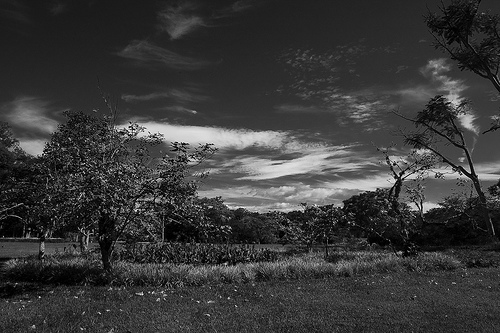
\includegraphics[scale=0.3]{img01.jpg}
    \caption{Imagem Original}
    \label{img1}
\end{figure}
\begin{figure}[!ht]
    \centering
    \includegraphics[scale=0.1]{histBefore.pdf}
    \vspace{-20pt}
    \caption{Histograma da Imagem Original}
    \label{histBefore}
\end{figure}
\begin{figure}[!ht]
    \centering
    \includegraphics[scale=0.3]{img01-final.jpg}
    \caption{Imagem com Contraste Alterado}
    \label{img1-f}
\end{figure}
\begin{figure}[!ht]
    \centering
    \includegraphics[scale=0.1]{histAfter.pdf}
    \vspace{-20pt}
    \caption{Histograma da Imagem Alterada}
    \label{histAfter}
\end{figure}




\subsection{Blur}
\begin{figure}[!htb]
    \centering
    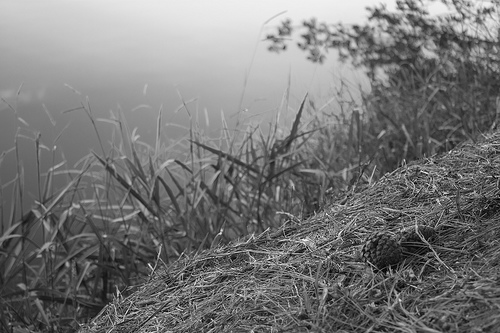
\includegraphics[scale=0.3]{img03.jpg}
    \caption{Imagem Original}
    \label{img3}
\end{figure}
\begin{figure}[!htb]
    \centering
    \includegraphics[scale=0.3]{img03-final.jpg}
    \caption{Imagem com filtro Blur}
    \label{img3-f}
\end{figure}






\subsection{Sharpenning}
\begin{figure}[!htb]
    \centering
    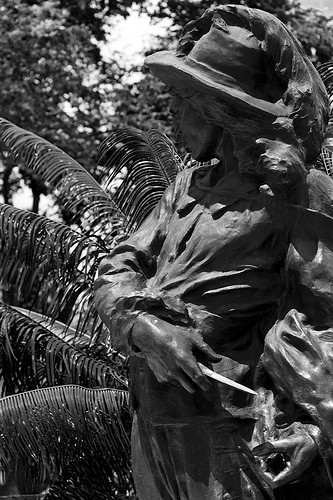
\includegraphics[scale=0.3]{img02.jpg}
    \caption{Imagem Original}
    \label{img5}
\end{figure}
\begin{figure}[!htb]
    \centering
    \includegraphics[scale=0.3]{intermediario.jpg}
    \caption{Imagem Intermediária após o Laplaciano}
    \label{interm}
\end{figure}
\begin{figure}[!htb]
    \centering
    \includegraphics[scale=0.3]{img02-final.jpg}
    \caption{Imagem com filtro Sharpenning}
    \label{img5-f}
\end{figure}

\end{document}
